\documentclass{article}
\usepackage{graphicx}
\usepackage[margin=1.5cm]{geometry}
\usepackage{amsmath}

\begin{document}
\twocolumn

\title{Monday warm-up: Kinematics III, and the Cross-Product}
\author{Prof. Jordan C. Hanson}

\maketitle

\begin{figure}
\centering
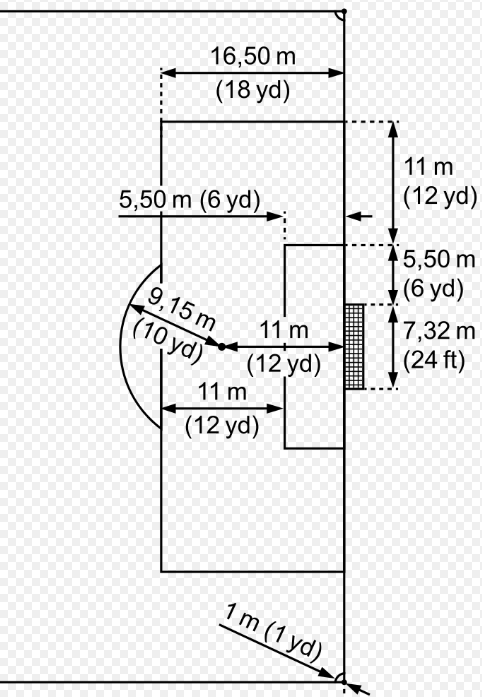
\includegraphics[width=0.2\textwidth]{figures/soccer_pitch.png}
\caption{\label{fig:1} A technical diagram of a football pitch.}
\end{figure}

\begin{figure}
\centering
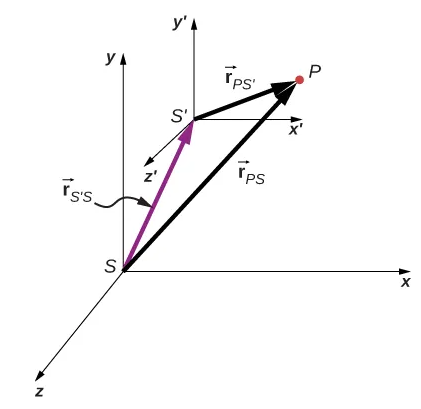
\includegraphics[width=0.33\textwidth]{figures/ref.png}
\caption{\label{fig:2} A point $P$ in two reference frames.}
\end{figure}

\section{Memory Bank}

\begin{enumerate}
\item The \textbf{cross-product}:
\begin{itemize}
\item $\hat{i} \times \hat{j} = \hat{k}$
\item $\hat{k} \times \hat{i} = \hat{j}$
\item $\hat{j} \times \hat{k} = \hat{i}$
\item Non-alphabetical order: multiply by -1. For example, $\hat{k} \times \hat{i} = -\hat{j}$
\item $\hat{i} \times \hat{i} = 0$, $\hat{j} \times \hat{j} = 0$, $\hat{k} \times \hat{k} = 0$
\end{itemize}
\end{enumerate}

\section{The Cross Product of Vectors}

\begin{enumerate}
\item Evaluate: (a) $\vec{v}_1 = -2 \hat{i} - 2 \hat{j}$, and $\vec{v}_2 = 2\hat{i} + 2\hat{j}$. (b) $\vec{v}_1 = 2 \hat{i} - 2 \hat{j}$, and $\vec{v}_2 = 2\hat{i} + 2\hat{j}$.\\ \vspace{0.5cm}
\end{enumerate}

\section{Kinematics III: Projectiles}

\begin{enumerate}
\item Consider Fig. \ref{fig:1}.  Suppose a soccer player must take a penalty kick from the outside corner of the penalty area towards the far goal post.  The distance to the goal line is 16.50 m, and the distance across the pitch is 11 m, plus 5.5 m, plus 7.32 m. (a) What is the straight-line distance from the ball to the far goal post? (b) The goal post top corner is 2.45 m above the ground.  If the player strikes the ball with an initial angle of 30 degrees above the xy-plane, is the initial velocity that causes it to reach the top corner of the goal? \\ \vspace{3.5cm}
\end{enumerate}

\section{Kinematics III: Relative motion}

\begin{enumerate}
\item Consider Fig. \ref{fig:2}.  Let $\vec{r}_{PS}$ be the position of a point $P$ in system $S$.  Let $\vec{r}_{PS'}$ be the position in $S$'.  Let $\vec{r}_{S'S}$ be the displacement from the origin of $S$ to $S$'.  (a) Show that 
\begin{equation}
\vec{r}_{PS} = \vec{r}_{PS'}+\vec{r}_{S'S} \label{eq:1}
\end{equation}
(b) Take the derivative of both sides of Eq. \ref{eq:1} to obtain the relationship between the relative velocities in reference frames $S$ and $S'$. (c) A truck is traveling south at a speed of 65 km/h toward an intersection. A car is traveling east toward the intersection at a speed of 85 km/h. What is the velocity of the car relative to the truck?
\end{enumerate}

\end{document}
